\documentclass[conference,a4paper]{IEEEtran}
\IEEEoverridecommandlockouts
\usepackage{cite}
\usepackage{amsmath,amssymb,amsfonts}
\usepackage{graphicx}
\usepackage{textcomp}
\usepackage{xcolor}
\usepackage{float}
\usepackage{url}
\usepackage[caption=false,font=footnotesize]{subfig}
\graphicspath{{../figures/}}

\def\BibTeX{{\rm B\kern-.05em{\sc i\kern-.025em b}\kern-.08em
    T\kern-.1667em\lower.7ex\hbox{E}\kern-.125emX}}

\makeatletter
\newcommand{\linebreakand}{%
  \end{@IEEEauthorhalign}
  \hfill\mbox{}\par
  \mbox{}\hfill\begin{@IEEEauthorhalign}
}
\makeatother

\begin{document}

\title{A Prototype Platform for Managing White--Light Solar Observations Integrating Embedded Acquisition and Web Consultation}

\author{
% \IEEEauthorblockN{Carlos Ben\'itez}
% \IEEEauthorblockA{\textit{Facultad de Ingenier\'ia}\\
% \textit{Universidad Nacional de Asunci\'on}\\
% Paraguay}
% \and
% \IEEEauthorblockN{Juan Cabral}
% \IEEEauthorblockA{\textit{Facultad de Ingenier\'ia}\\
% \textit{Universidad Nacional de Asunci\'on}\\
% Paraguay}
% \and
% \IEEEauthorblockN{Diego Stalder}
% \IEEEauthorblockA{\textit{Facultad de Ingenier\'ia}\\
% \textit{Universidad Nacional de Asunci\'on}\\
% Paraguay}
% \linebreakand
% \IEEEauthorblockN{Jos\'e Mar\'ia G\'omez}
% \IEEEauthorblockA{\textit{Facultad Polit\'ecnica}\\
% \textit{Universidad Nacional de Asunci\'on}\\
% Paraguay}
% \and
% \IEEEauthorblockN{Christian Schaerer}
% \IEEEauthorblockA{\textit{Facultad Polit\'ecnica}\\
% \textit{Universidad Nacional de Asunci\'on}\\
% Paraguay}
% \and
% \IEEEauthorblockN{Jes\'us N\'u\~nez}
% \IEEEauthorblockA{\textit{Facultad Polit\'ecnica}\\
% \textit{Universidad Nacional de Asunci\'on}\\
% Paraguay}
}

\maketitle

\begin{abstract}
Small academic observatories that perform white-light solar imaging frequently rely on separate tools for capture, metadata registration, storage, and later consultation. This fragmentation limits the preservation of provenance between the acquired image, capture parameters, processing state, and database record. This paper presents an integrated prototype platform that connects a heliographic acquisition prototype, a Raspberry Pi 5 embedded node, a Supabase/PostgreSQL persistence layer, and a web platform. The workflow starts with a Vixen refractor, Herschel-wedge attenuation, neutral-density filtering, and a ZWO ASI174MM Mini camera. The embedded node controls acquisition, stores and preprocesses observations locally, and synchronizes prepared records when connectivity is available. Supabase stores full-disk images, metadata, identifiers, operational captures, and object paths, while the web platform supports image loading, metadata review, historical consultation, and visualization. The resulting architecture maintains traceable, portable, and repeatable observation records from acquisition to consultation.
\end{abstract}

\begin{IEEEkeywords}
Solar observations, embedded systems, Raspberry Pi 5, Supabase, scientific instrumentation, web platform, data management.
\end{IEEEkeywords}

\section{Introduction}

White-light observations of the photosphere provide records of sunspot morphology, location, and temporal persistence that complement operational solar-region reports~\cite{mcintosh1990classification,noaaSRS}. In small academic observatories, however, capture, metadata registration, storage, processing, and consultation are commonly handled with separate tools. This operational fragmentation makes it difficult to preserve the relationship between the original image, acquisition parameters, derived crops, classifications, and observation history.

The gap addressed in this work is the lack of a unified acquisition and management platform for white-light solar observations in small academic observatories. The objective is to organize optical acquisition, local preprocessing, structured persistence, web access, and observation management into one workflow that preserves provenance from capture to consultation.

Ground-based observatories provide the operational reference for this objective. Long-running stations such as the Uccle Solar Equatorial Table (USET) combine white-light, H$\alpha$, and CaII K observations with visual annotation, digital acquisition, and catalog preservation, while synoptic networks such as the Global Oscillation Network Group (GONG) illustrate the value of distributed monitoring for temporal continuity~\cite{robUSET2026,sidcGroundObservations2026,nsoGONG2026}. These examples demonstrate that observation records require explicit links among image data, metadata, provenance, and later consultation. For small observatories, the same requirement must be addressed under field conditions that include seeing, clouds, dust, and occasional occlusions.

The proposed architecture connects a heliographic acquisition prototype, a Supabase-based storage and metadata layer, and a web platform for visualization, processing, and historical consultation. The remainder of the article follows the data path through the system: architecture, acquisition hardware and firmware, local preparation of observations, database organization, web interface, validation, and conclusions.

\section{End-to-End System Architecture}

% The system is organized as a directed data flow from acquisition to consultation. The optical acquisition prototype produces a full-disk image, the Raspberry Pi 5 node prepares and stores the observation locally, Supabase receives the synchronized object and relational metadata, and the web platform exposes registered records for visualization and consultation. Each layer has a distinct responsibility so that the image file, acquisition context, processing state, and database path remain associated throughout the workflow.

The embedded node is housed in the 3D-printed enclosure shown in Figure~\ref{fig:cad-open-enclosure}. The enclosure was manufactured in polylactic acid (PLA), selected for its low cost, dimensional stability during printing, and accessibility for rapid prototyping. Its base is compatible with a standard 1/4--20 photographic thread for attachment to a tripod or telescope mount, and its ventilation openings preserve airflow for the active cooler while reducing direct dust exposure of the internal electronics.

\begin{figure}[t]
    \centering
    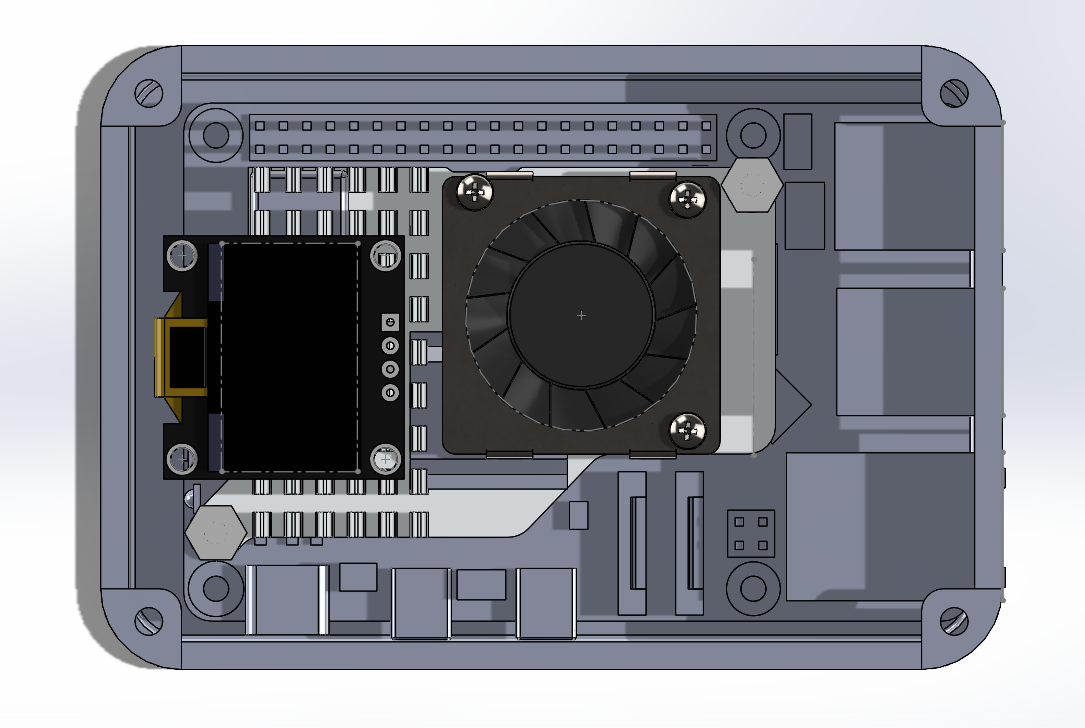
\includegraphics[width=\linewidth]{cad/case_open.png}
    \caption{CAD view of the custom 3D enclosure used to organize and protect the embedded acquisition node.}
    \label{fig:cad-open-enclosure}
\end{figure}

\begin{figure*}[t]
    \centering
    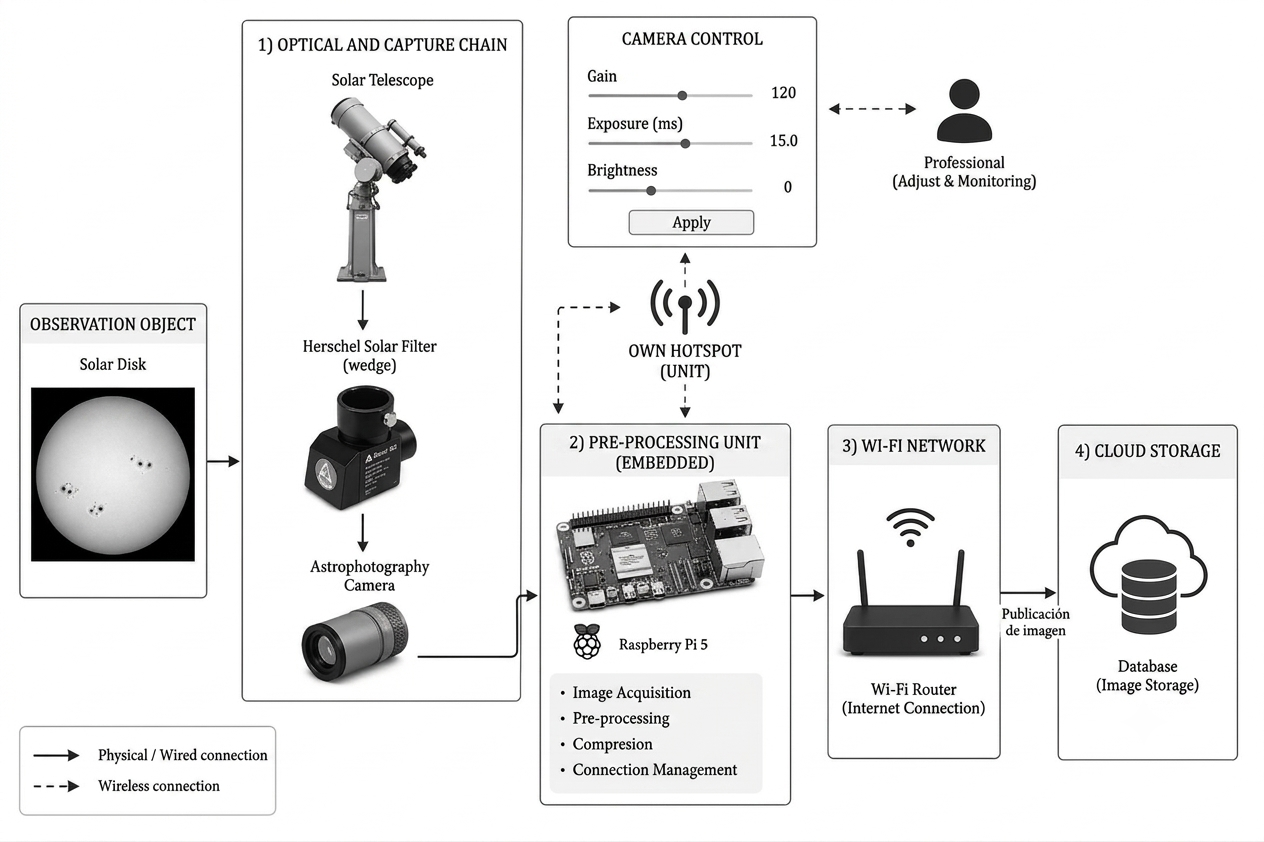
\includegraphics[width=0.92\textwidth]{hw/module2.png}
    \caption{Embedded preprocessing workflow of the acquisition prototype.}
    \label{fig:embedded-dual-workflow}
\end{figure*}

Figure~\ref{fig:embedded-dual-workflow} details the operational stages of the acquisition prototype. First, the camera acquisition stage receives the full-disk solar image from the optical train and transfers the frame to the Raspberry Pi 5 node. Second, the local operation stage exposes a browser-based panel for configuring capture parameters and monitoring the acquisition state near the telescope. Third, the dual-connectivity stage allows the node either to provide a local access point for field configuration or to join an available network as a client for data publication. Fourth, the local-preparation stage stores, preprocesses, and packages the observation with metadata. Finally, the publication stage synchronizes the prepared image object and relational metadata when connectivity is available.

\begin{figure*}[t]
    \centering
    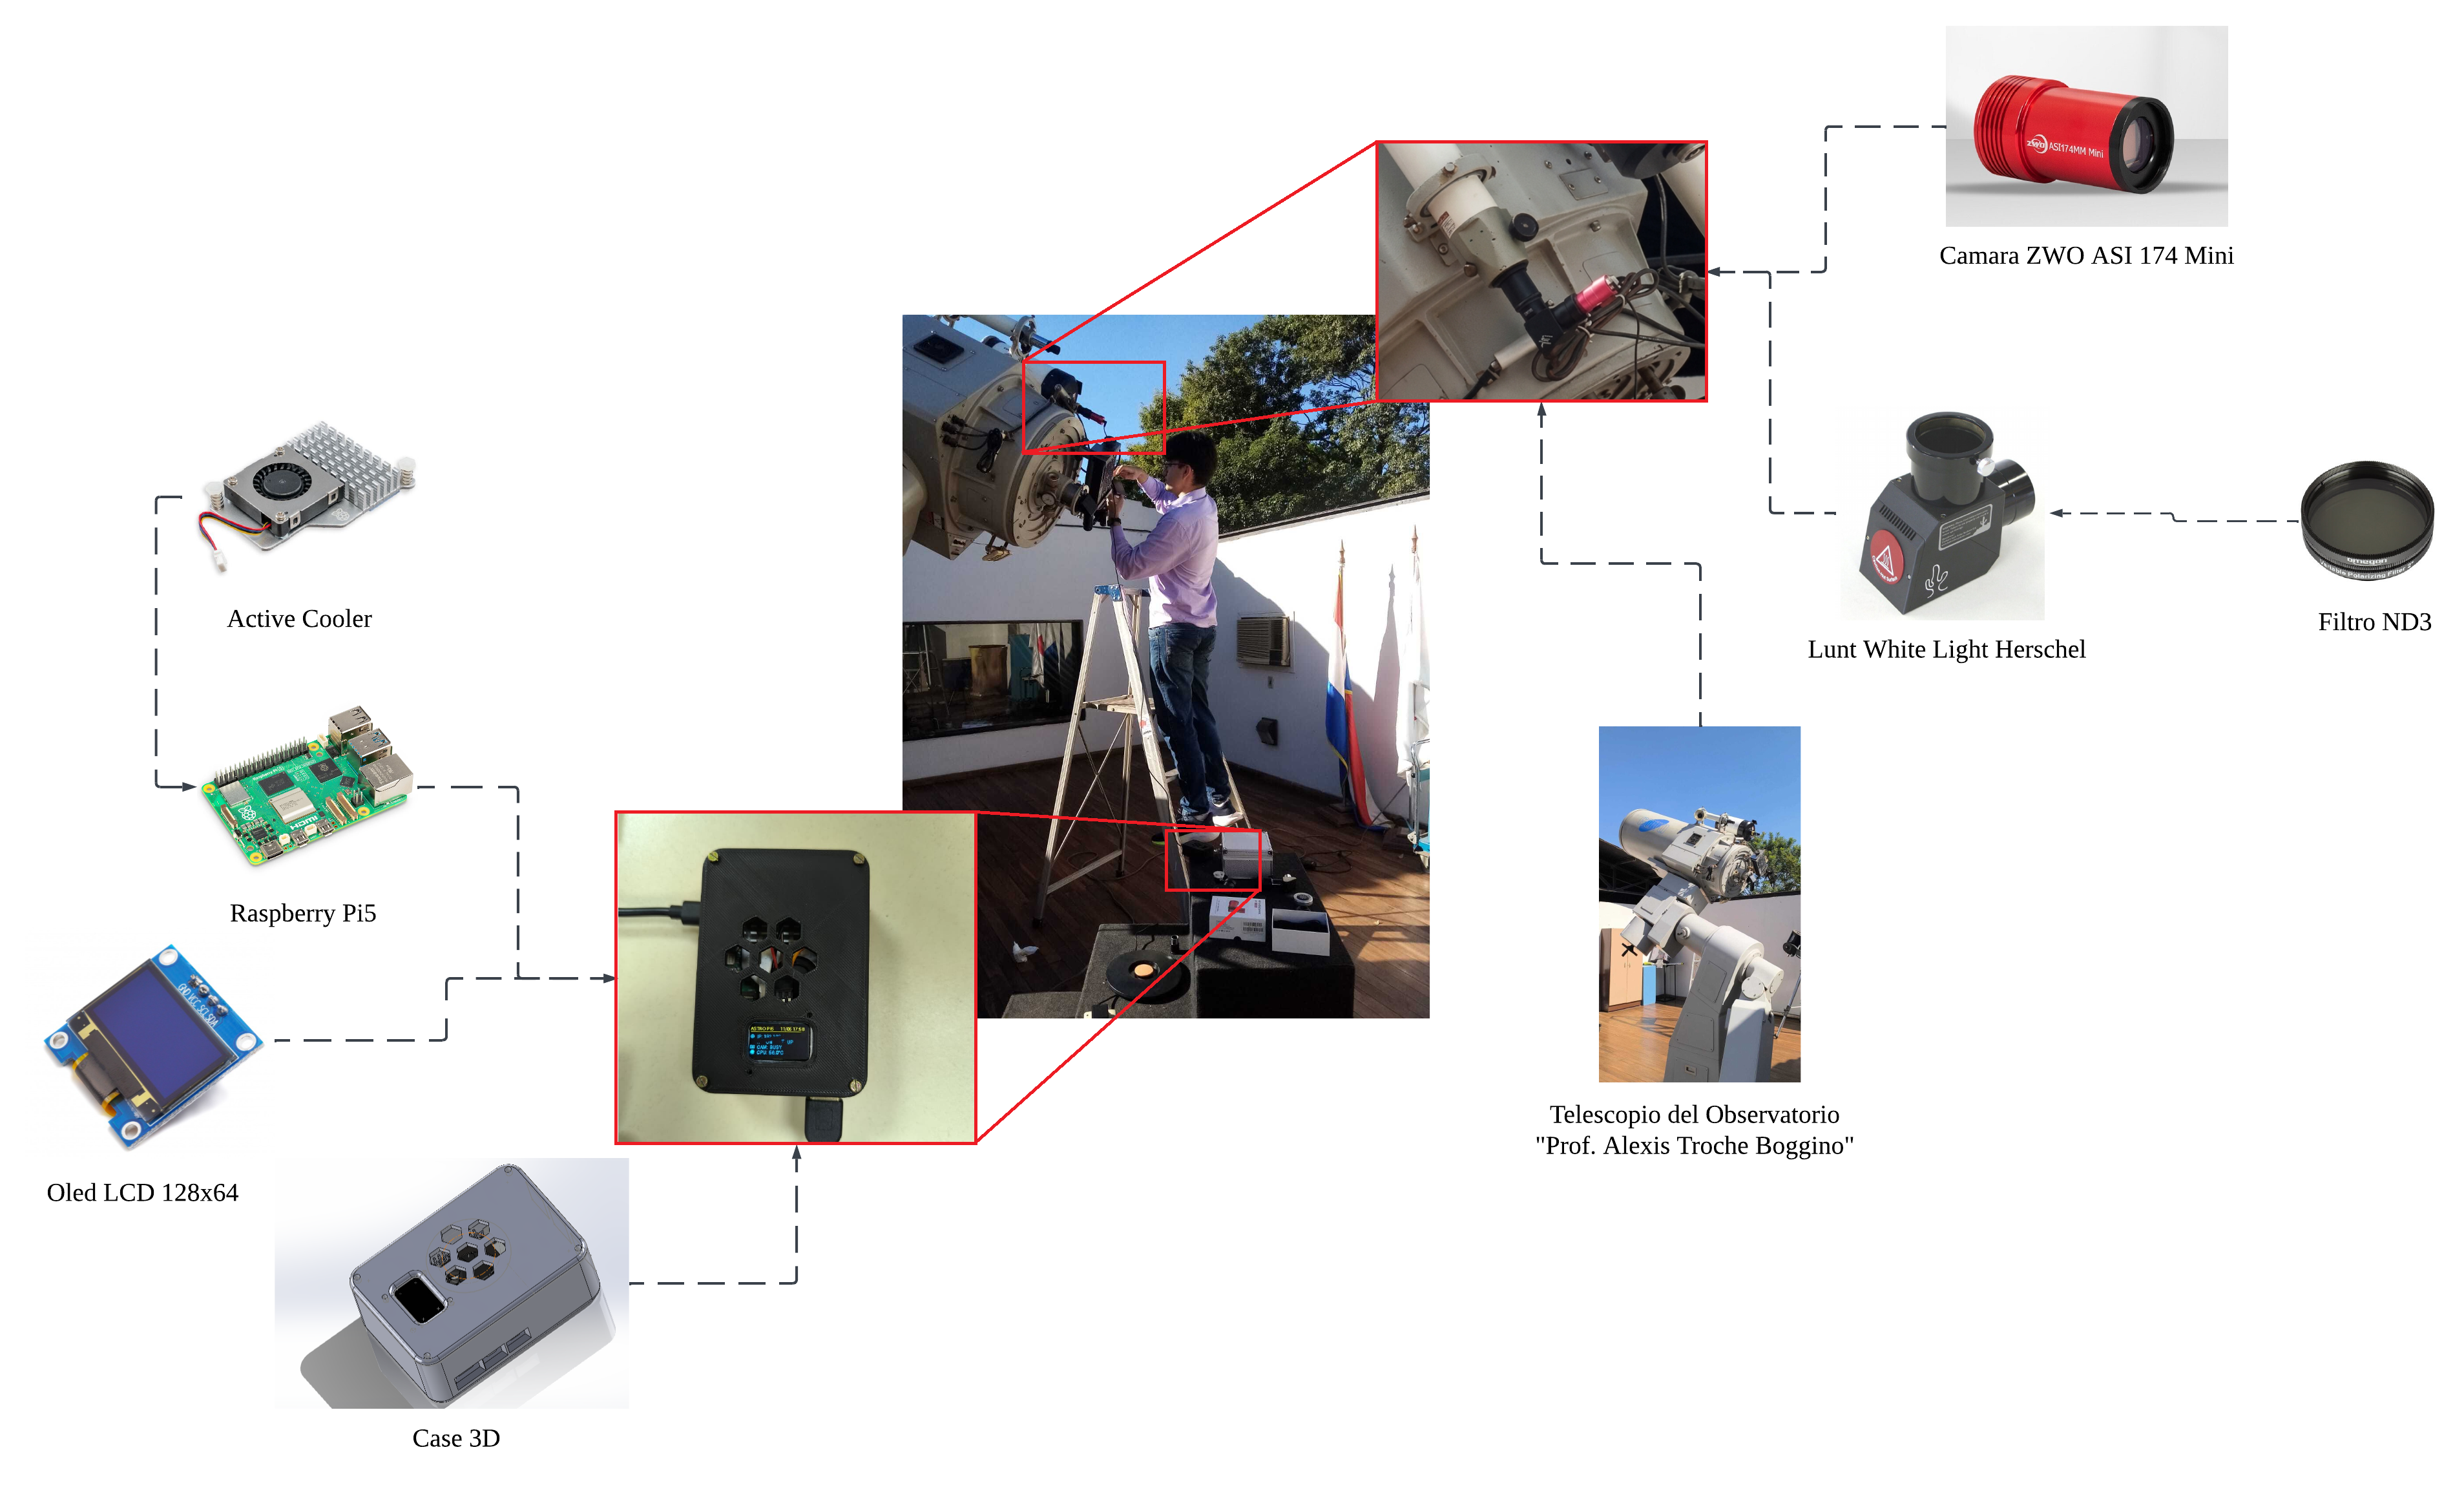
\includegraphics[width=0.92\textwidth]{hw/hw_diagram.png}
    \caption{Hardware-level organization of the local observation prototype.}
    \label{fig:hardware-architecture}
\end{figure*}

Figure~\ref{fig:hardware-architecture} maps these responsibilities to the physical and software blocks of the prototype. The following section starts at the acquisition layer, where optical attenuation, sensor choice, embedded control, and field operation define the input conditions for the rest of the workflow.

\begin{figure*}[t]
    \centering
    \subfloat[Electrical connection diagram.\label{fig:electrical-connections}]{%
        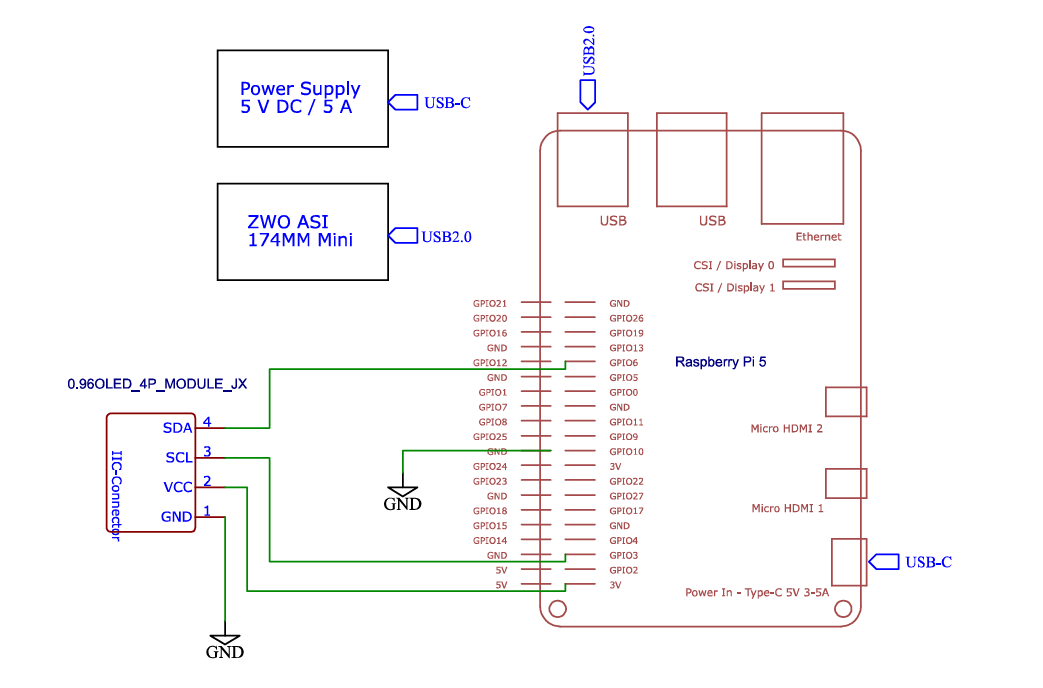
\includegraphics[width=0.58\textwidth]{hw/electric.png}}
    \hfill
    \subfloat[Optical acquisition prototype.\label{fig:acquisition-module}]{%
        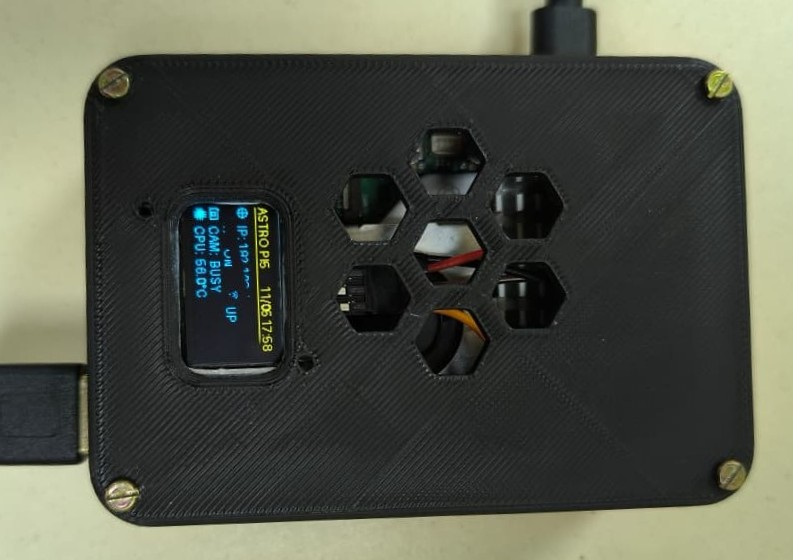
\includegraphics[width=0.34\textwidth]{hw/obs_module.jpeg}}
    \caption{Electrical and optical components of the embedded white-light solar observation prototype.}
    \label{fig:electrical-optical-components}
\end{figure*}

\section{Heliographic Acquisition Prototype}

This section describes the acquisition prototype through four aspects that determine the input conditions of the observation workflow. The optical chain defines how the solar image is formed and attenuated before reaching the sensor. The sensor selection explains the camera characteristics used for white-light capture. The embedded control and field-parameter subsection describes the Raspberry Pi 5 node, physical interconnections, power requirements, and documented acquisition settings. The firmware and dual-mode operation subsection then explains how camera control and local/network operation are coordinated during field use.

\subsection{Optical Chain}

The acquisition prototype provides the white-light solar images that enter the processing workflow. It uses a Vixen refractor telescope with aperture $D=60$ mm and focal length $F=420$ mm. This compact refractor was adopted as a portable and mechanically simple optical platform for early validation, reducing alignment complexity while preserving a full-disk field suitable for local observation campaigns. Solar attenuation is performed with a Herschel prism, or Herschel wedge, together with neutral-density filtering~\cite{luntWhiteLightWedges2026}. In this configuration, the wedge provides the primary energy rejection for refractor-based white-light observation, and additional brightness control is treated as a secondary adjustment after the primary attenuation stage~\cite{luntWhiteLightWedges2026,baaderHerschelUsage2026,luntPolarizerWedge2026}. The resulting optical path supports observation of photospheric structures and supplies the full-disk images used by later processing stages.


\subsection{Sensor Selection}

Image capture is performed with a ZWO ASI174MM Mini monochromatic astrophotography camera~\cite{zwoASI174Manual2025}. Its 1/1.2-inch Sony IMX174 sensor, $1936\times1216$ pixel format, 5.86~$\mu$m pixels, 12-bit conversion, and compact mini body match the mechanical and sampling constraints of the prototype~\cite{zwoASI174Manual2025,zwoGuideCameras2025}. The Sony Pregius global-shutter architecture reduces temporal distortion during solar imaging, especially when short exposures and variable seeing are involved~\cite{sonyPregiusGlobalShutter}. The monochromatic sensor avoids color-filter interpolation and preserves spatial detail for sunspot observation, which is consistent with scientific monochrome imaging workflows~\cite{janesick2001scientific,fossum1997cmos}.


\subsection{Embedded Control and Field Parameters}

The acquisition prototype is controlled by a Raspberry Pi 5 embedded node~\cite{raspberryPi5Docs2026}. This board provides the CPU, memory, WiFi connectivity, software support, and power characteristics required by the portable station; alternative single-board computers were considered during the design analysis~\cite{raspberryPi5Docs2026,jetsonOrinNanoGuide2026,orangePi5Plus2026,rock5bDocs2026}. The documented assembly includes active cooling, an OLED status display connected through I2C, a custom 3D-printed protective enclosure, and a local web panel for field operation.

Figure~\ref{fig:electrical-connections} details the physical interconnection of the embedded node. The ZWO ASI174MM Mini is connected to the Raspberry Pi 5 through USB, while the OLED display uses the I2C bus on the GPIO header: SDA on GPIO2/pin~3, SCL on GPIO3/pin~5, 3.3~V on pin~1, and common ground on pin~6. The active cooler is mounted directly on the BCM2712 processor and is powered from the 5~V rail; if fan-speed control is enabled, a GPIO line can be reserved for PWM or tachometer supervision.

The complete system, including the Raspberry Pi 5, ZWO camera, OLED display, and active cooling, consumes approximately 12~W (5~V, 2.4~A) during a typical capture and preprocessing session. A 5~V/5~A external supply is recommended to provide adequate current margin during USB transfer, fan operation, and network synchronization. For field operation without grid power, the same 5~V rail can be supplied by a 20,000~mAh USB-C battery, providing an estimated autonomy of about 8~h under the measured operating load.


The local application documented in the thesis is identified as \texttt{pi5-observatory}. During the reported capture session, the configurable acquisition parameters included frames per second, binning, gain, image width, image height, exposure, and sensor temperature. Table~\ref{tab:capture-parameters} summarizes the values used for the documented 2026-05-05 capture.

\begin{table}[t]
\caption{Acquisition parameters used during the documented solar capture.}
\label{tab:capture-parameters}
\centering
\begin{tabular}{ll}
\hline
\textbf{Parameter} & \textbf{Value} \\
\hline
Local application & \texttt{pi5-observatory} \\
Version & 1.0 \\
Frame rate & 15 FPS \\
Sensor temperature & 36.7~$^\circ$C \\
Binning & 1 \\
Gain & 1 \\
Image size & $1936\times1216$ px \\
Exposure & 500~$\mu$s \\
\hline
\end{tabular}
\end{table}



\subsection{Firmware and Dual-Mode Operation}

The firmware layer completes the acquisition chain by exposing the camera to the local application. It runs on Ubuntu~24 on the Raspberry Pi 5 and uses the ZWO ASI SDK for camera access~\cite{zwoASILinuxManual}. At runtime, the acquisition service detects the ASI174MM Mini, initializes the camera interface, and applies exposure, gain, image-format, region-of-interest, and capture-sequence settings without requiring manual camera operation.

The capture software is organized around a camera worker that isolates hardware access from the local web panel. The worker initializes the ASI camera, applies the selected acquisition parameters, allocates the SDK image buffer, and converts the raw frame into a numerical image representation for local processing. Preview frames are encoded as JPEG for low-latency visualization in the browser, while observation frames are retained with their acquisition parameters for storage and later synchronization. This separation avoids coupling the user interface to USB camera timing and allows the acquisition loop to continue even when the browser is disconnected or refreshed.

Field operation uses two network modes. The Raspberry Pi 5 can create a local WiFi hotspot for configuration and monitoring near the instrument, or it can join an available WiFi network as a client for publication. This capability separates field control from Internet availability: the local panel exposes camera availability, network state, frame rate, binning, gain, exposure, image dimensions, and capture status, while observations remain in local storage with a pending state until synchronization can be attempted~\cite{nmcliHotspot2026}.


\section{Local Preprocessing and Observation Packaging}

After acquisition, the embedded node prepares the observation for persistence. The local sequence includes file storage, basic preprocessing, metadata association, and construction of a record for later synchronization. Each package links the image file, capture timestamp, device context, camera parameters, processing state, and storage path. It can be created offline, inspected through the local interface, retried after failures, and transmitted later without losing the relationship between the image and its acquisition context.

Local preprocessing includes camera-calibration routines for sensor and optical artifacts. Bias, dark, and flat frames can be captured and applied automatically to reduce fixed-pattern noise, dark-current contribution, and illumination nonuniformity. The calibration parameters are stored in the local file system and applied to each image before synchronization, so the observation record preserves both the corrected image and the acquisition context used to generate it.

Image preparation also applies a logarithmic stretch to the normalized pixel intensity $I\in[0,1]$,
\begin{equation}
    I' = \frac{\log(1 + \alpha I)}{\log(1 + \alpha)},
\end{equation}
where $\alpha>0$ controls the compression of high-intensity disk values and the expansion of lower-intensity regions. This transformation addresses the low contrast that sunspot structures can present against the surrounding photosphere, particularly in field observations affected by atmospheric seeing and changes in illumination. The computation can be executed on the Raspberry Pi 5 during local preparation without adding a separate workstation.

Synchronization is decoupled from capture. A successful capture first produces a complete local record; publication to Supabase is then attempted as a later step that uploads the image object, writes the relational metadata, and marks the local item as synchronized only after both operations complete. This condition defines the atomicity of the publication step at the application level. If the network or remote service is unavailable, the observation remains queued locally and can be retried without repeating the optical acquisition. This sequence reduces the risk of partial records in which an image exists without its metadata, or metadata points to a missing object. Figure~\ref{fig:solar-capture-20260505} shows one full-disk image generated by this pipeline during the prototype validation session.

\begin{figure}[t]
    \centering
    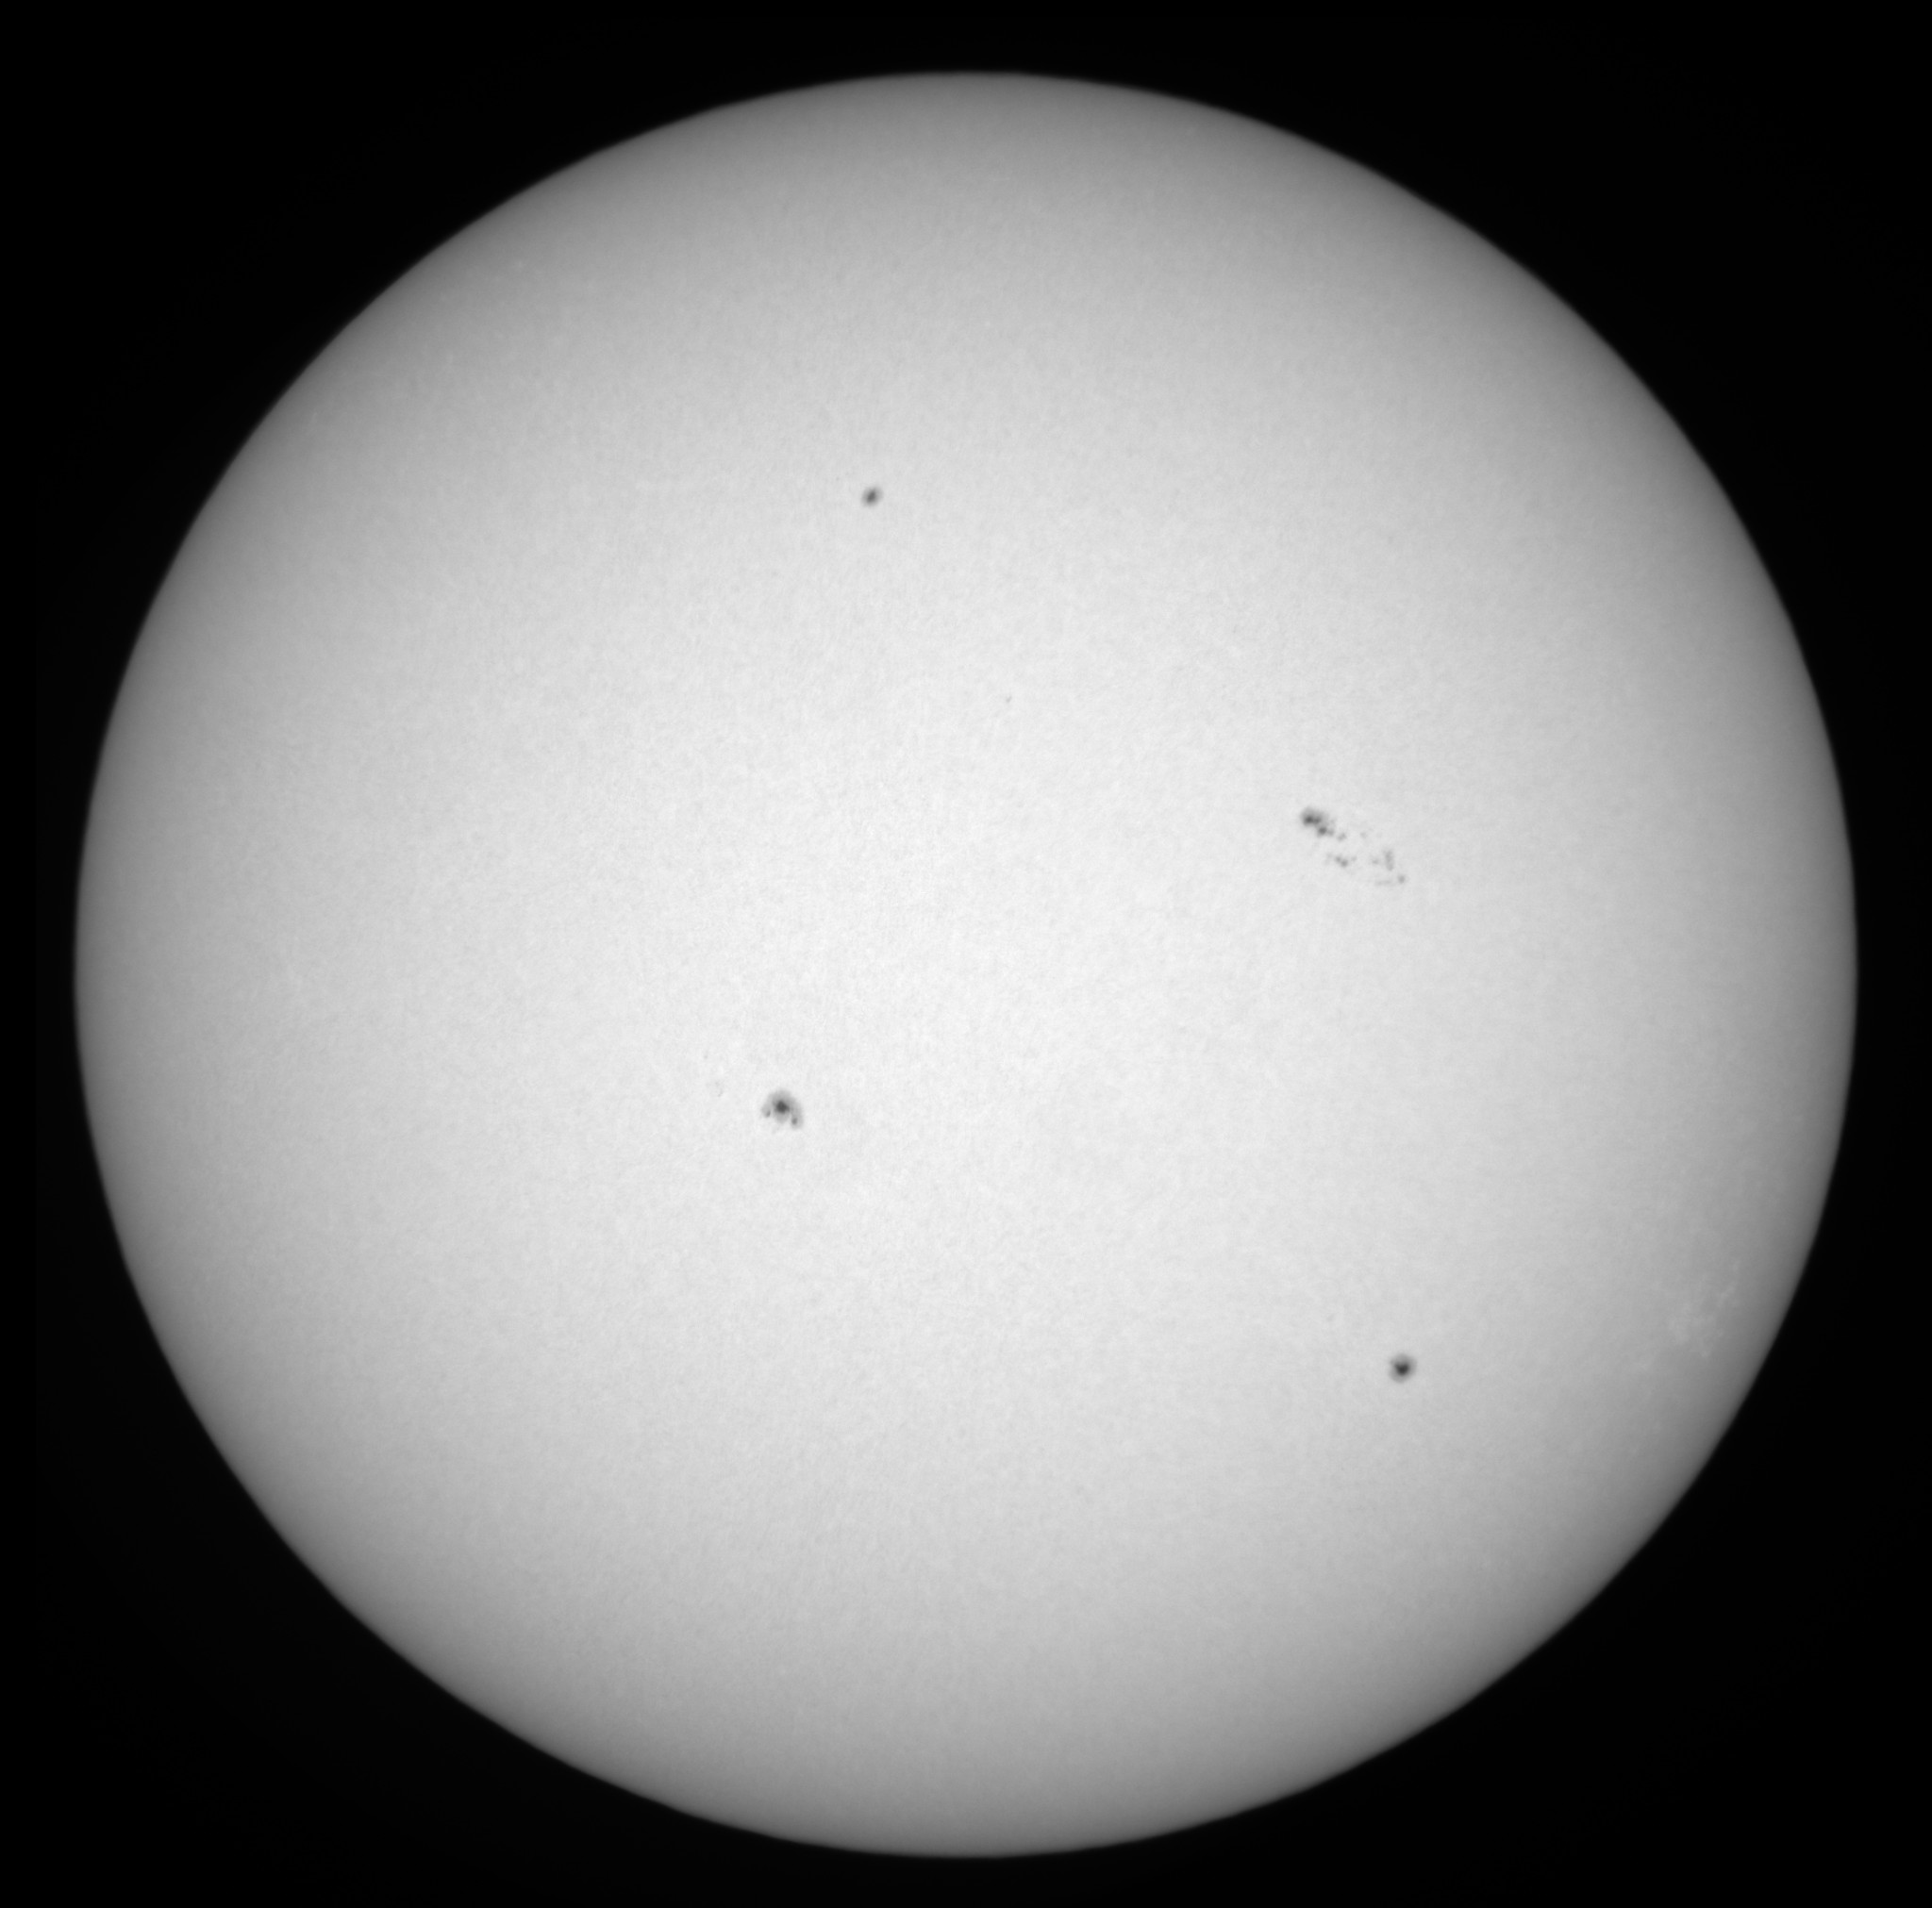
\includegraphics[width=0.86\linewidth]{implementacion_final/obs_20260505_225301_568d2c89.jpg}
    \caption{Solar full-disk image captured with the local observation prototype during the 2026-05-05 validation session.}
    \label{fig:solar-capture-20260505}
\end{figure}

\section{Supabase Data Architecture}

The persistence layer is deployed in Supabase over PostgreSQL. It separates binary object storage from relational metadata: image files are stored in Supabase Storage, including a private \texttt{snapshots} bucket, while PostgreSQL stores identifiers, object paths, observation metadata, and relationships among records.

\begin{table*}[t]
\caption{Main persistence entities in the Supabase/PostgreSQL layer.}
\label{tab:supabase-entities}
\centering
\begin{tabular}{p{0.18\textwidth}p{0.36\textwidth}p{0.38\textwidth}}
\hline
\textbf{Entity} & \textbf{Stored content} & \textbf{Relation in the model} \\
\hline
\texttt{datasets} & Dataset identifier, version, description, label file, and aggregate counts & Root collection for full-disk images and derived crops \\
\texttt{full\_disk\_images} & File name, bucket, object path, observation date, dimensions, NOAA list, and metadata & References one dataset and groups extracted sunspot crops \\
\texttt{sunspot\_crops} & Crop path, crop index, classifications, coordinates, area, NOAA identifier, and confidence values & References one dataset and one source full-disk image \\
Operational captures & Recent observation metadata, acquisition parameters, processing state, and storage path & Links field captures with synchronized storage objects \\
Supabase Storage & Full-disk images, crops, and private snapshot objects & Stores binary files referenced by PostgreSQL object paths \\
\hline
\end{tabular}
\end{table*}

The relational model is organized around three historical entities. The \texttt{datasets} table is the root entity and identifies each collection with a UUID, name, version, description, label file, and counts of crops and full-disk images. The \texttt{full\_disk\_images} table references a dataset and stores each solar disk image with its file name, storage bucket, object path, observation date, dimensions, crop count, NOAA list, and additional metadata in \texttt{jsonb} format. The \texttt{sunspot\_crops} table references both the dataset and the source full-disk image, so each extracted region remains linked to its original observation.

The crop table fields are grouped into four categories. Identification fields include crop name, object path, crop index, observation date, and source-image reference. Classification fields include the Zurich--McIntosh components, complete McIntosh combination, magnetic class, and model-related outputs. Geometry fields include heliographic coordinates, Carrington longitude, detection center, original crop size, extension, and area. Operational metadata include the NOAA identifier, reported spot count, storage information, and confidence values. Including Zurich--McIntosh fields preserves compatibility with a standard sunspot-group morphology vocabulary, while NOAA and coordinate fields preserve links to operational reports~\cite{mcintosh1990classification,noaaSRS}. The same structure can relate local records to external products such as SDO/HMI observations when those sources are used for comparison or dataset construction~\cite{scherrer2012hmi,noaaSRS}.

Recent operational captures are represented as synchronized records rather than as isolated uploads: the storage object path, observation metadata, acquisition parameters, and processing state are kept together. The database design includes uniqueness restrictions to avoid duplicated datasets, full-disk files, and crop records. Row-level access control can be applied to operational tables so authenticated web operations can retrieve and register observations without exposing private storage objects directly.

\section{Web Platform}

The web platform provides remote access after observations have been published. Unlike the local Raspberry Pi 5 panel, which controls acquisition near the telescope, the web platform focuses on registered data: image display, metadata review, historical consultation, and visualization of observation records.

\begin{figure*}[t]
    \centering
    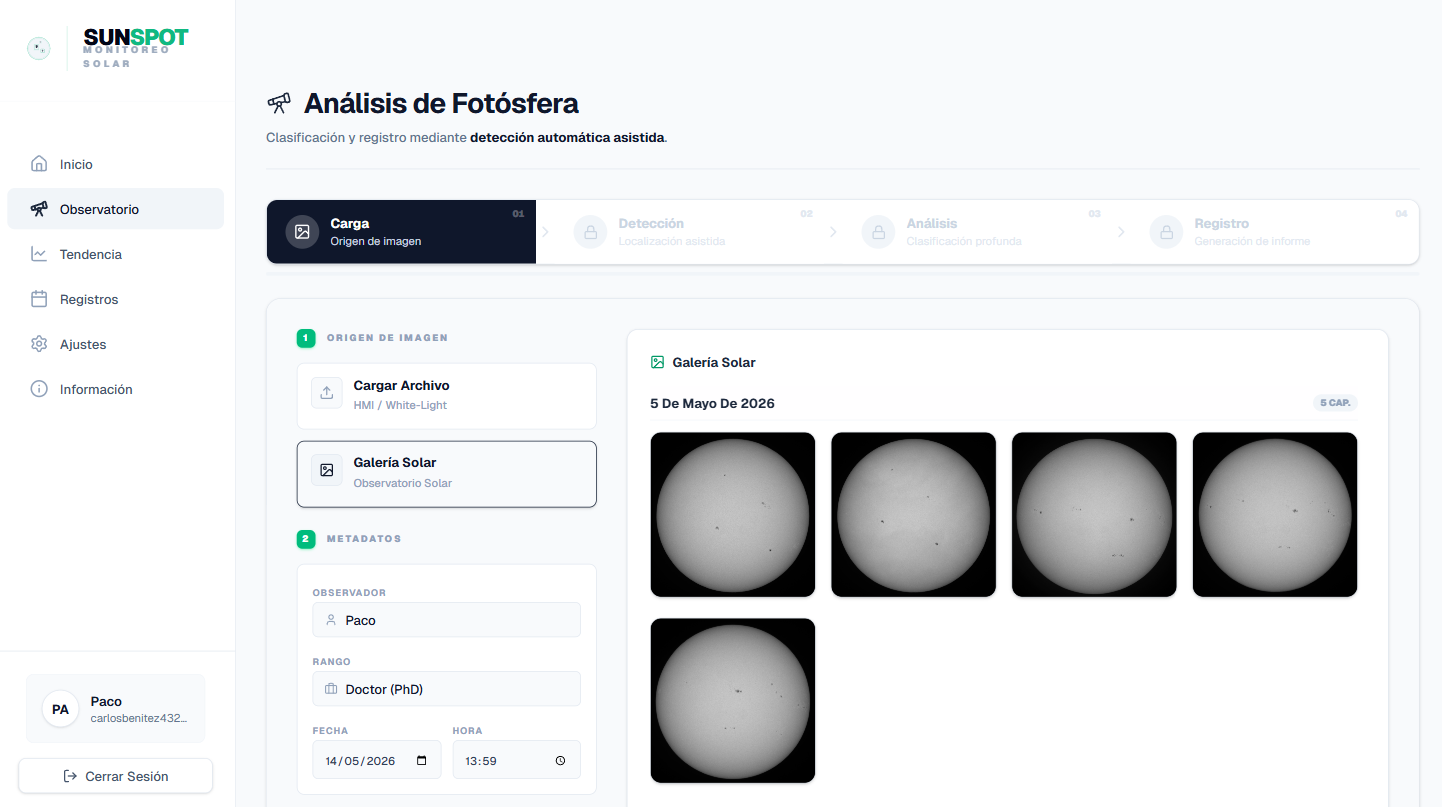
\includegraphics[width=0.92\textwidth]{web/upload.png}
    \caption{Web interface for uploading or selecting a solar observation before registration or consultation.}
    \label{fig:web-upload}
\end{figure*}

The platform is organized into interface and data/service layers. The interface layer displays solar disk images and observation records. The data/service layer communicates with PostgreSQL/Supabase to retrieve historical observations, register new records, and resolve storage paths. In the upload and selection view shown in Fig.~\ref{fig:web-upload}, the user associates a new or existing solar image with the metadata required for registration. After registration, the interface allows the user to inspect the image, review associated metadata, and consult historical records without duplicating the acquisition functions performed by the local panel.



\section{Operational Validation}

Validation was performed on the integrated acquisition and data-management prototype under the documented WiFi and active-cooling conditions. Table~\ref{tab:operational-metrics} groups the measured values into three categories: timing metrics for capture, storage, preprocessing, and synchronization; resource metrics for CPU and RAM use; and the thermal metric after a 25~min operating interval.

\begin{table}[t]
\caption{Operational metrics of the Raspberry Pi 5 acquisition node.}
\label{tab:operational-metrics}
\centering
\begin{tabular}{lc}
\hline
\textbf{Metric} & \textbf{Value} \\
\hline
Individual image capture & 420~ms \\
Local microSD storage & 180~ms \\
Capture + local storage & 600~ms \\
Basic preprocessing per image & 1350~ms \\
Supabase synchronization & 3800~ms/image \\
Average CPU use & 38\% \\
Maximum CPU use in preprocessing & 72\% \\
Local service RAM use & 3.3~GB \\
Temperature after 25 min & 57~$^\circ$C \\
\hline
\end{tabular}
\end{table}

The timing values indicate the measured duration of each stage in a representative operating session: individual frame capture, local write to microSD, combined capture and storage, basic preprocessing, and synchronization to Supabase. The resource values report average CPU use, maximum CPU use during preprocessing, and RAM use of the local service. During the thermal test at an ambient temperature of 25~$^\circ$C, the processor temperature stabilized at 57~$^\circ$C after 25~min of continuous capture and preprocessing, remaining below the 80~$^\circ$C thermal-throttling threshold. Without active cooling, the processor temperature exceeded 70~$^\circ$C in less than 10~min, which supports the use of forced airflow for sustained observation sessions.

The system was also evaluated across five observation sessions at the Observatorio Astron\'omico ``**** (blind peer review rule)''. A successful automatic acquisition was defined as a capture completed without manual intervention and followed by local storage of the observation record. Under this criterion, the success rate was above 90\%. Failed attempts were mainly associated with adverse sky conditions, especially dense cloud cover; the acquisition service handles these cases through a retry timer before attempting the next capture.

Commercial telescope-computer solutions such as the PrimaLuceLab EAGLE6 and closed acquisition ecosystems such as ZWO ASIAIR provide a reference point for positioning the prototype~\cite{primaluceEagle62026,zwoASIAIR2026}. The comparison is not used as a performance benchmark; it frames the prototype as a reproducible academic platform for acquisition, traceability, and web consultation, rather than as a replacement for professional solar-monitoring infrastructure.

\section{Conclusion}

This paper presents an integrated prototype platform for managing local white-light solar observations in academic observatories. The validated workflow connects optical acquisition, embedded preparation, asynchronous synchronization, Supabase persistence, and web-based consultation while maintaining a single observation record across these stages.

The main contribution is the traceable organization of the acquisition and data-management process. Images captured at the telescope remain associated with metadata, local storage state, database paths, and later consultation. This structure provides a practical basis for distributed acquisition, structured storage, and remote access in observatories with limited infrastructure.

The current prototype has hardware and validation constraints. Sustained operation depends on active cooling, spatial resolution is limited by the 60~mm aperture telescope, and dust accumulation on the optical train or sensor window requires periodic maintenance and recalibration. These constraints indicate that the prototype is intended to complement, not replace, professional solar-monitoring facilities. Future work should extend observational campaigns, incorporate additional solar-data sources, and evaluate image-processing or predictive components as layers above the acquisition and data-management architecture.


\bibliographystyle{IEEEtran}
\bibliography{references}

\end{document}
